\documentclass{article}

% Language setting
% Replace `english' with e.g. `spanish' to change the document language
\usepackage[english]{babel}

% Set page size and margins
% Replace `letterpaper' with`a4paper' for UK/EU standard size
\usepackage[letterpaper,landscape, top=2cm,bottom=2cm,left=1cm,right=1cm,marginparwidth=1.75cm]{geometry}

% Useful packages
\usepackage{amsmath}
\usepackage{graphicx}
\usepackage[colorlinks=true, allcolors=blue]{hyperref}

\title{Evaluation of Cohen 1998's Biphasic Model}
\author{Rahul Yerrabelli, Alexander Spector}

\begin{document}
\maketitle

\section{Introduction}
Taking Cohen's biphasic model and comparing Cohen's analytic solution with our numerical results. \cite{cohen1998}. As there is a discrepancy, take the case of $C_1=C_2$ to prove which is correct.

\section{Key property of $C_1=C_2$}

$\text{If $C_1=C_2$ (because $\nu_{31}=\pm\sqrt{1/2}$), then:}$
\begin{align}
\frac{\widetilde{F(s)}}{\tilde{\varepsilon}_{zz}(s)}
&=\frac{C_{1} I_{0}\left[\sqrt{s}\right]-C_{2} C_{0} \frac{I_{1}\left[\sqrt{s}\right]}{\sqrt{s}}}{I_{0}\left[\sqrt{s}\right]-C_{0} \frac{I_{1}\left[\sqrt{s}\right]}{\sqrt{s}}}  \\
&= C_{1} \frac{I_{0}\left[\sqrt{s}\right]-C_{0} \frac{I_{1}\left[\sqrt{s}\right]}{\sqrt{s}}}{I_{0}\left[\sqrt{s}\right]-C_{0} \frac{I_{1}\left[\sqrt{s}\right]}{\sqrt{s}}}  \\
&= C_1 \\
&\quad \textbf{ if } \underbrace{s\neq0}_{\text{Already known } \text{invalid point}} \textbf{ and }
\underbrace{I_{0}\left[\sqrt{s}\right] \neq C_{0} \frac{I_{1}\left[\sqrt{s}\right]}{\sqrt{s}}}_{\text{Tricky condition, } \text{will return to it}}
\end{align}

$\text{If those conditions are satisfied, then:}$

\begin{align}
f(t) &= \ilaplace{C_1 \tilde{\varepsilon}_{zz}(s)} \\
&= C_1 \ilaplace{\dot{\varepsilon}_{0} t_{g} \left( \frac{1-\exp \left(-s \frac{t_{0}}{t_{g}}\right)}{s^{2}} \right)} \\
&= C_1 \varepsilon_{zz}(t)
\end{align}

It will be proven later that this is satisfied only with $\nu_{31}=0.5$. See in Figure \ref{fig:C1EqualsC2} (corresponding to \ref{tab:C1EqualsC2}) that the numerical solution is a perfect ramp as expected at this $\nu_{31}$ value, unlike Cohen's analytic solution.


\begin{figure}[h]
\centering
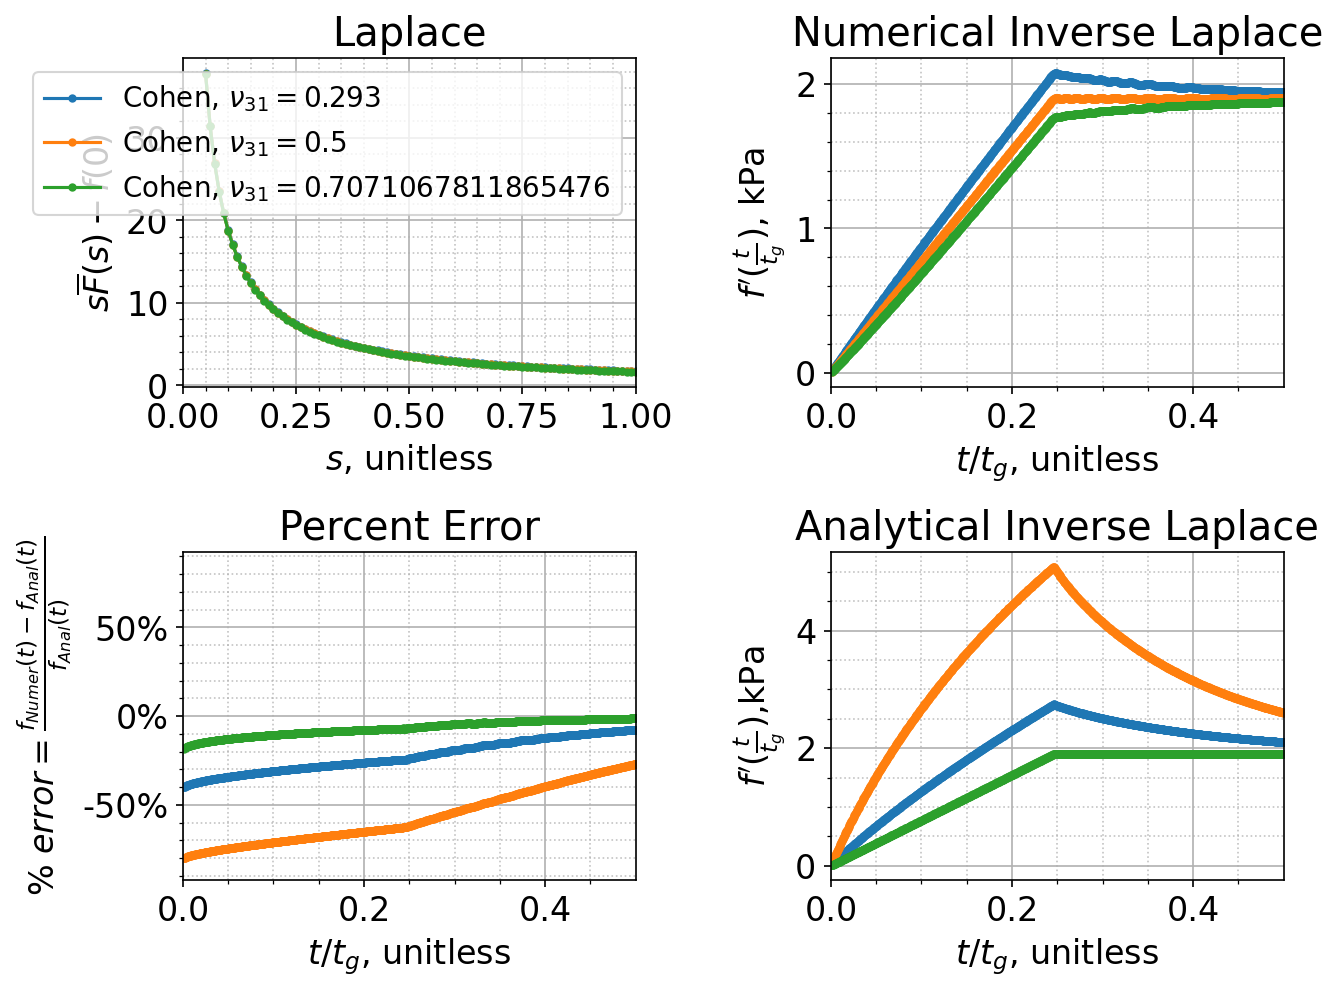
\includegraphics[width=0.6\textwidth]{PlotsWhenC1=C2.png}
\caption{\label{fig:C1EqualsC2} Note that the numerical solution is a perfect ramp at $\nu_{31}=0.5$ as expected, unlike Cohen's proposed analytic solution.}
\end{figure}

\begin{table}[!ht]
    \centering
    \caption{\label{tab:C1EqualsC2} Paramaters for lines plotted}
    \begin{tabular}{|l|l|l|l|l|l|l|l|l|l|l|l|l|l|l|l|l|l|}
    \hline
        ~ & $t_0/t_g$ & tg & $\dot{\varepsilon{}}$ & E1 & E3 & v21 & v31 & $\Delta$1 & $\Delta$2 & $\Delta$3 & C11 & C12 & C13 & C33 & C0 & C1 & C2  \\ \hline
        Line \#1 & 0.246184 & 40.62 & 0.01 & 8.5 & 19 & 0.75 & 0.293 & 0.173188 & 0.549482 & 2.628 & 26.968415 & 22.111272 & 14.38 & 27.426 & 0.18 & 9.555 & 27.055  \\ \hline
        Line \#2 & 0.246184 & 40.62 & 0.01 & 8.5 & 19 & 0.75 & 0.5 & 0.026316 & 0.507519 & 9.6428 & 163.928 & 159.071429 & 161.5 & 180.5 & 0.0296 & 7.823 & 7.823  \\ \hline
        Line \#3 & 0.246184 & 40.62 & 0.01 & 8.5 & 19 & 0.75 & 0.707 & -0.197368 & 0.443609 & 4e-16 & -19.104762 & -23.961905 & -30.45 & -24.067 & -0.254 & 6.302 & 19.790 \\ \hline
    \end{tabular}
\end{table}

\section{Proof 1 that $C_1\!=\!C_2 \iff \nu_{31}\!=\!0.5$}

Set $C_1$ = $C_2$:
\begin{align}
\overbrace{\frac{C_{11} +C_{12} -4C_{13} +2C_{33}}{C_{11}-C_{12}}}^{C_1}
 &= \overbrace{ 2 \frac{C_{33} \left( C_{11} - C_{12} \right) + C_{11} \left( C_{11}+C_{12}-4C_{13} \right) + 2C_{13}^2 }{\left( C_{11}-C_{12} \right)^2} }^{C_2}  \\
\left( C_{11}-C_{12} \right) \left( C_{11} +C_{12} -4C_{13} +2C_{33} \right) &= 2 C_{33} \left( C_{11} - C_{12} \right) + 2 C_{11} \left( C_{11}+C_{12}-4C_{13} \right) + 4 C_{13}^2   \\
\left( C_{11}-C_{12} \right) \left( C_{11} +C_{12} -4C_{13} \right) &=  2 C_{11} \left( C_{11}+C_{12}-4C_{13} \right) + 4 C_{13}^2  \\
-\left( C_{11}+C_{12} \right) \left( C_{11} +C_{12} -4C_{13} \right) &=  4 C_{13}^2  \\
- \frac{E_1}{\Delta_1} \cdot \frac{E_1 \left(1-4\nu_{31} \right)}{\Delta_1} &= 4 \left( \frac{E_1 \nu_{31}}{\Delta_1} \right)^2 \\
\left( \frac{E_1}{\Delta_1} \right)^2 \left(4\nu_{31}-1 \right) &= 4 \nu_{31}^2 \left( \frac{E_1}{\Delta_1} \right)^2 \\
\left( 4 \nu_{31}^2 -4 \nu_{31} +1 \right) \left( \frac{E_1}{\Delta_1} \right)^2 &= 0 \\
\left( 2 \nu_{31} -1 \right)^2 \left( \frac{E_1}{\Delta_1} \right)^2 &= 0 \\
\end{align}


\text{Knowing } E_1=0 \text{ is impossible } \text{as then } C_{11}=C_{12}=0 \\
\text{Thus, only one pair of solutions remains: } \\ 
\begin{align}
2 \nu_{31} -1 &= 0 \\
\nu_{31} &= \frac{1}{2}  \iff C_1=C_2
\end{align}

\noindent\rule{20cm}{0.8pt}

\newpage 
\section{Proof 2 that $C_1\!=\!C_2 \iff \nu_{31}\!=\!0.5$}

Strategy: get $C_1$ - $C_2$ directly in terms of constants ($\nu_{21}$, $\nu_{31}$, $E_1$, $E_3$), then set them equal each other.

\subsection{Getting C11, C12, etc directly in terms of parameters}


\begin{align}
C_{11}
&=\frac{E_1 \cdot \left( 1-\nu_{31}^2 \frac{E_1}{E_3} \right)}{ \left(1+\nu_{21}\right) \cdot \Delta_1} \\
&=\frac{E_1 \cdot \left( 1-\nu_{31}^2 \frac{E_1}{E_3} \right)}{ \left(1+\nu_{21}\right) \left( 1-\nu_{21}-2\nu_{31}^2\frac{E_1}{E_3} \right) } \\
C_{12}
&=\frac{E_1 \cdot \left( \nu_{21}+\nu_{31}^2 \frac{E_1}{E_3} \right)}{ \left(1+\nu_{21}\right) \cdot \Delta_1} \\
&=\frac{E_1 \cdot \left( \nu_{21}+\nu_{31}^2 \frac{E_1}{E_3} \right)}{ \left(1+\nu_{21}\right)  \left( 1-\nu_{21}-2\nu_{31}^2\frac{E_1}{E_3} \right) } \\
C_{13}
&=\frac{E_1 \nu_{31}}{ \Delta_1} \\
&=\frac{E_1 \nu_{31}}{ 1-\nu_{21}-2\nu_{31}^2\frac{E_1}{E_3} } \\
C_{33}
&=E_3 \cdot \left( 1 + \frac{  2\nu_{31}^2 \frac{E_1}{E_3}}{\Delta_1} \right)
= \frac{ \Delta_1 E_3 + 2\nu_{31}^2 E_1}{\Delta_1} \\
&=E_3 \cdot \left( 1 + \frac{  2\nu_{31}^2 \frac{E_1}{E_3}}{ 1-\nu_{21}-2\nu_{31}^2\frac{E_1}{E_3} } \right) \\
&= \frac{ \left( 1-\nu_{21}-2\nu_{31}^2\frac{E_1}{E_3} \right) E_3 + 2 \nu_{31}^2 E_1}{ 1-\nu_{21}-2\nu_{31}^2\frac{E_1}{E_3} }  \\
&= \frac{ E_3 \cdot \left( 1-\nu_{21} \right) }{ 1-\nu_{21}-2\nu_{31}^2\frac{E_1}{E_3} }  \\
\end{align}
\noindent\rule{8cm}{0.4pt}

\subsection{Combinations of C11, C12, etc}
\begin{align}
C_{11}-C_{12}
&=\frac{E_1}{1+\nu_{21}} \\
\\
C_{11}+C_{12}
&=\frac{E_1}{\Delta_1} \\
&=\frac{E_1}{ 1-\nu_{21}-2\nu_{31}^2\frac{E_1}{E_3} } \\
\\
C_{13} 
&= \frac{E_1 \nu_{31}}{ 1-\nu_{21}-2\nu_{31}^2\frac{E_1}{E_3} }  \\
\\
C_{33} 
&= \frac{ E_3 \cdot \left( 1-\nu_{21} \right) }{ 1-\nu_{21}-2\nu_{31}^2\frac{E_1}{E_3} }  \\
\\
C_{11}+C_{12}-4C_{13} 
&= \frac{E_1 \left(1-4\nu_{31} \right)}{\Delta_1}  \\
&= \frac{E_1 \cdot \left(1-4\nu_{31} \right)}{ 1-\nu_{21}-2\nu_{31}^2\frac{E_1}{E_3} }  \\
\\
C_{11}+C_{12}-4C_{13}+2C_{33} 
&= \frac{E_1 \left(1-4\nu_{31} \right) + 2 E_3 \left( 1-\nu_{21} \right) }{ 1-\nu_{21}-2\nu_{31}^2\frac{E_1}{E_3} }  \\
&= \frac{E_1+2E_3 -4 E_1 \nu_{31} - 2E_3 \nu_{21} }{ 1-\nu_{21}-2\nu_{31}^2\frac{E_1}{E_3} }  \\
\end{align}

\noindent\rule{8cm}{0.4pt}

\subsection{Getting $C_0, C_1,$ directly in terms of parameters}

\begin{align}
C_0 
&= \frac{C_{11} - C_{12}}{C_{11}} = \frac{\Delta_1}{1-\nu_{31}^2 \frac{E_1}{E_3}} = \frac{1-\nu_{21}-2\nu_{31}^2\frac{E_1}{E_3}}{1-\nu_{31}^2 \frac{E_1}{E_3}} \\
\\
C_1 
&= \frac{C_{11} +C_{12} -4C_{13} +2C_{33}}{C_{11}-C_{12}}   \\
&= \frac{\left( 1+\nu_{21} \right) \left( 1-4\nu_{31} + 2 \frac{E_3}{E_1} \left( 1-\nu_{21} \right) \right) }{ \left( 1-\nu_{21}-2\nu_{31}^2\frac{E_1}{E_3} \right) }  \\
\\
C_2 
&= 2 \frac{C_{33} \left( C_{11} - C_{12} \right) + C_{11} \left( C_{11}+C_{12}-4C_{13} \right) + 2C_{13}^2 }{\left( C_{11}-C_{12} \right)^2}   \\
&= 2 \frac{ \left( \frac{ E_3 \cdot \left( 1-\nu_{21} \right) }{ 1-\nu_{21}-2\nu_{31}^2\frac{E_1}{E_3} } \right) \left( \frac{E_1}{1+\nu_{21}} \right) + \left( \frac{E_1 \cdot \left( 1-\nu_{31}^2 \frac{E_1}{E_3} \right)}{ \left(1+\nu_{21}\right) \left( 1-\nu_{21}-2\nu_{31}^2\frac{E_1}{E_3} \right) } \right)  \left( \frac{E_1 \cdot \left(1-4\nu_{31} \right)}{ 1-\nu_{21}-2\nu_{31}^2\frac{E_1}{E_3} } \right) + 2 \left( \frac{E_1 \nu_{31}}{ 1-\nu_{21}-2\nu_{31}^2\frac{E_1}{E_3} } \right)^2 }{\left( \frac{E_1}{1+\nu_{21}} \right)^2}   \\
&= 2 \frac{ E_3 E_1 \left( 1-\nu_{21} \right) \left( 1-\nu_{21}-2\nu_{31}^2\frac{E_1}{E_3}  \right) + E_1^2 \cdot \left( 1-\nu_{31}^2 \frac{E_1}{E_3} \right) \left(1-4\nu_{31} \right)+ 2 E_1^2 \nu_{31}^2 \left( 1+\nu_{21} \right) }{\left( \frac{E_1}{1+\nu_{21}} \right)^2 \left( 1-\nu_{21}-2\nu_{31}^2\frac{E_1}{E_3} \right)^2 \left( 1+\nu_{21} \right) }   \\
&= 2 \frac{ \frac{E_3}{E_1} \left( 1-\nu_{21} \right) \left( 1-\nu_{21}-2\nu_{31}^2\frac{E_1}{E_3}  \right) + \left( 1-\nu_{31}^2 \frac{E_1}{E_3} \right) \left(1-4\nu_{31} \right)+ 2\nu_{31}^2 \left( 1+\nu_{21} \right) }{ \frac{ \left( 1-\nu_{21}-2\nu_{31}^2\frac{E_1}{E_3} \right)^2 }{1+\nu_{21}} }   \\
&= 2 \frac{ \frac{E_3}{E_1} \left( 1-\nu_{21}^2 \right) \left( 1-\nu_{21}-2\nu_{31}^2\frac{E_1}{E_3}  \right) + \left( 1-\nu_{31}^2 \frac{E_1}{E_3} \right) \left(1-4\nu_{31} \right) \left(1+\nu_{21}\right) + 2\nu_{31}^2 \left( 1+\nu_{21} \right)^2 }{ \left( 1-\nu_{21}-2\nu_{31}^2\frac{E_1}{E_3} \right)^2 }   \\
&= 2 \left( 1+\nu_{21} \right) \frac{ \frac{E_3}{E_1} \left( 1-\nu_{21} \right) \left( 1-\nu_{21}-2\nu_{31}^2\frac{E_1}{E_3}  \right) + \left( 1-\nu_{31}^2 \frac{E_1}{E_3} \right) \left(1-4\nu_{31} \right)+ 2\nu_{31}^2 \left( 1+\nu_{21} \right) }{ \left( 1-\nu_{21}-2\nu_{31}^2\frac{E_1}{E_3} \right)^2 }   \\
\end{align}


\noindent\rule{8cm}{0.4pt}

\subsection{Solve for $C_1$=$C_2$}
Knowing:
\begin{align}
C_0 &= \frac{1-\nu_{21}-2\nu_{31}^2\frac{E_1}{E_3}}{1-\nu_{31}^2 \frac{E_1}{E_3}} \\
\\
C_1 &= \frac{\left( 1+\nu_{21} \right) \left( 1-4\nu_{31} + 2 \frac{E_3}{E_1} \left( 1-\nu_{21} \right) \right) }{ 1-\nu_{21}-2\nu_{31}^2\frac{E_1}{E_3} }  \\
\\
C_2 
&= 2 \frac{ \frac{E_3}{E_1} \left( 1-\nu_{21}^2 \right) \left( 1-\nu_{21}-2\nu_{31}^2\frac{E_1}{E_3}  \right) + \left( 1-\nu_{31}^2 \frac{E_1}{E_3} \right) \left(1-4\nu_{31} \right) \left(1+\nu_{21}\right) + 2\nu_{31}^2 \left( 1+\nu_{21} \right)^2 }{ \left( 1-\nu_{21}-2\nu_{31}^2\frac{E_1}{E_3} \right)^2 }   \\
\end{align}

We want to solve for $C_1$=$C_2$:

\begin{align*}
\overbrace{\frac{\left( 1+\nu_{21} \right) \left( 1-4\nu_{31} + 2 \frac{E_3}{E_1} \left( 1-\nu_{21} \right) \right) }{ 1-\nu_{21}-2\nu_{31}^2\frac{E_1}{E_3} } }^{C_1}
&= 
\overbrace{
2 \frac{
    \scriptstyle{
\frac{E_3}{E_1} \left( 1-\nu_{21}^2 \right) \left( 1-\nu_{21}-2\nu_{31}^2\frac{E_1}{E_3}  \right) + \left( 1-\nu_{31}^2 \frac{E_1}{E_3} \right) \left(1-4\nu_{31} \right) \left(1+\nu_{21}\right) + 2\nu_{31}^2 \left( 1+\nu_{21} \right)^2}
}{
\left( 1-\nu_{21}-2\nu_{31}^2\frac{E_1}{E_3} \right)^2 
} }^{C_2}  \tag{A}  \\
\end{align*}

\begin{align*} 
\small{ \text{Multiply both sides by }}& \scriptstyle{\left( 1-\nu_{21}-2\nu_{31}^2\frac{E_1}{E_3} \right)^2} \\
{
\left( 1+\nu_{21} \right) \left( 1-4\nu_{31} + 2 \frac{E_3}{E_1} \left( 1-\nu_{21} \right) \right)  \left( 1-\nu_{21}-2\nu_{31}^2\frac{E_1}{E_3}  \right) }
&= { 2 \frac{E_3}{E_1} \left( 1-\nu_{21}^2 \right) \left( 1-\nu_{21}-2\nu_{31}^2\frac{E_1}{E_3}  \right) + 2 \left( 1-\nu_{31}^2 \frac{E_1}{E_3} \right) \left(1-4\nu_{31} \right) \left(1+\nu_{21}\right) + 4\nu_{31}^2 \left( 1+\nu_{21} \right)^2  } \\
\small{\text{Divide both sides by }}&\scriptscriptstyle{1+\nu_{21}}
\\ {
\left( 1-4\nu_{31} + 2 \frac{E_3}{E_1} \left( 1-\nu_{21} \right) \right)  \left( 1-\nu_{21}-2\nu_{31}^2\frac{E_1}{E_3}  \right) }
&= {
\underbrace{2 \frac{E_3}{E_1} \left( 1-\nu_{21} \right) \left( 1-\nu_{21}-2\nu_{31}^2\frac{E_1}{E_3}  \right)}_{\text{Move to lefthand side}} + 2\left( 1-\nu_{31}^2 \frac{E_1}{E_3} \right) \left(1-4\nu_{31} \right) + 4\nu_{31}^2 \left( 1+\nu_{21} \right) }
\tag{B} \\
\left( 1-4\nu_{31} \right)  \left( 1-\nu_{21}-2\nu_{31}^2\frac{E_1}{E_3}  \right)
&=
\underbrace{2\left( 1-\nu_{31}^2 \frac{E_1}{E_3} \right) \left(1-4\nu_{31} \right)}_{\text{Move to lefthand side}} + 4\nu_{31}^2 \left( 1+\nu_{21} \right) 
\tag{C} \\
\left( 1-4\nu_{31} \right)  \left( 1-\nu_{21}-2\nu_{31}^2\frac{E_1}{E_3} -2\left( 1-\nu_{31}^2 \frac{E_1}{E_3} \right) \right)
&=
4\nu_{31}^2 \left( 1+\nu_{21} \right) 
\tag{D} \\
\left( 1-4\nu_{31} \right)  \left( -1- \nu_{21}\right) &= 4\nu_{31}^2 \left( 1+\nu_{21} \right) 
\tag{E} \\
-\left( 1-4\nu_{31} \right) \left(1+\nu_{21}\right)  &= 4\nu_{31}^2 \left( 1+\nu_{21} \right)  
\tag{F} \\
-\left( 1-4\nu_{31} +4\nu_{31}^2 \right) \left(1+\nu_{21}\right)  &= 0 
\tag{G}  \\
-\left( 4\nu_{31}^2-4\nu_{31}+1 \right) \left(1+\nu_{21}\right)  &= 0 
\tag{H} \\
-\left( 2\nu_{31}-1 \right)^2 \left(1+\nu_{21}\right)  &= 0   
\tag{I} \\
-\left( 2\nu_{31}-1 \right)^2 \left(1+\nu_{21}\right)  &= \left( C_1-C_2 \right) \overbrace{ \times \frac{\left( 1-\nu_{21}-2\nu_{31}^2\frac{E_1}{E_3}  \right)^2}{ 1+\nu_{21} } }^{\text{Multiplications/divisions } \text{done to get to this step}} \\
-\frac{ \left( 2\nu_{31}-1 \right)^2 \left(1+\nu_{21}\right)^2 }{\left( 1-\nu_{21}-2\nu_{31}^2\frac{E_1}{E_3}  \right)^2} &= C_1-C_2   
\end{align*}



\begin{gather*}
\boxed{
C_2-C_1 = \left( \frac{ \left( 2\nu_{31}-1 \right) \left(1+\nu_{21}\right) }{1-\nu_{21}-2\nu_{31}^2\frac{E_1}{E_3}  } \right)^2    }
\tag{J} \\
\end{gather*}



\text{Since }  $\nu_{21}\!=\!-1 \implies C_{11} \text{ and } C_{12}$ \text{ are undefined, } \text{we know $C_{11}=C_{12}$ has only one solution remaining: }


\boxed{
C_1=C_2 \iff \nu_{31}=0.5 \\
\text{assuming } 1-\nu_{21}-2\nu_{31}^2\frac{E_1}{E_3} \neq 0
} 
\\
\noindent\rule{8cm}{0.4pt}



\end{document}